\documentclass[12pt]{report}
\usepackage[utf8]{inputenc}

\usepackage[czech]{babel}
\usepackage{hyperref}
\usepackage{graphicx} 
\usepackage{float}
\usepackage{blindtext}
\usepackage{enumitem}
\usepackage{scrextend}


\usepackage{enumitem}
\usepackage{subcaption} 
\usepackage{float}


\title{Správa skladového systému}
\author{Jan Kohlíček}

\begin{document}

\begin{titlepage}
\begin{flushleft} 
{
\includegraphics[width=.5\textwidth]{../images/fav_logo.jpg}\\[3cm]}
\end{flushleft}
\begin{center}

{\Large KIV/MBKZ - Semestrální práce }
\\[0.3cm]
{\Huge Správa skladového systému}
\vspace{1.7cm}

{\Large Jan Kohlíček - A17N0075P}\\
\vspace{0.2cm}
{\normalsize kohl@students.zcu.cz }
\vfill
{\large \today}
\end{center}
\end{titlepage}

\tableofcontents
\thispagestyle{empty}



\chapter{Zadání}
\setcounter{page}{1}

Úkolem bude rozšířit mobilní aplikaci pro správu skladového systému. Kompletní dokumentace skladového systému je zde: \url{https://github.com/kohlicekjan/BPINI/blob/master/docs/bpini/BPINI.pdf}

První rozšíření se bude vázat ke změně autentizace, aktuálně se používá \texttt{HTTP Basic auth} a nahradit by ho měl bezpečnější protokol pro autentizaci \texttt{OAuth 2.0}.

Další rozšíření bude umožnovat vyhledávat položky skladu, uživatele a zařízení.
Také se musí změnit způsob propojení tagu se skladovou položkou, aktuálně se používá \texttt{Spinner}, pro velké množství skladových položek velmi nevhodné.  

Poslední rozšíření bude v duchu oprav chyb a drobných úprav pro lepší uživatelskou přívětivost.  


\chapter{Programátorská dokumentace}
	Vývoj mobilní aplikace probíhal nativně v \texttt{Javě} pro \texttt{Android 6.0}.
	Pro zrychlení vývoje jsem použil knihovnu \texttt{Butter Knife}. Její hlavní účel je eliminovat používání metody \texttt{findViewById} pomocí \texttt{property injection @BindView}.
	\texttt{@BindView} do jeho parametru stačí zadat \texttt{ID} požadované komponenty a knihovna \texttt{Butter Knife} automaticky inicializuje \texttt{atribut}. Tímto způsobem jsem dosáhl větší přehlednosti v kódu.
\\\\
Aby aplikace mohla správně fungovat potřebuje tato práva:
\begin{itemize}[noitemsep]
\item [-] INTERNET - umožňuje aplikacím otevřít síťové sokety.
\item [-] ACCESS\_NETWORK\_STATE - umožňuje přístup k informacím o síti.
\item [-] NFC - umožňuje provádět \texttt{I/O} operace přes \texttt{NFC}.
\end{itemize}	
		
\section{Grafické rozhraní}
Do grafického rozhraní jsem zavedl několik vylepšení. Na procházení velkého množství dat byla použita elegantní technika \texttt{infinite scroll}, bez nutnosti čekání se načte další stránka. Princip je jednoduchý, zatímco uživatel skroluje, další obsah je automaticky načítán. Pro rychlé nalezení konkrétních dat, se používá standardní vyhledávání v \texttt{Toolbaru}, které zajišťuje komponenta \texttt{SearchView}.
				
Tlačítka jako Uložit, Přihlásit, atd. jsou umístěna v komponentě \texttt{Toolbar}, což je z důvodu dlouhých formulářů, aby nemusel uživatel skrolovat. Takto je tlačítko stále k dispozici.
	
Pro znázornění \texttt{loadingu} byly použity komponenty \texttt{ProgressDialog} a \texttt{ProgressBar}.
\texttt{ProgressBar} se zobrazí při čekání na data od serveru.
\texttt{ProgressDialog} při odesílání dat nejde zrušit kvůli tomu, aby se zabránilo přerušení nebo opětovné operaci. Dialog se zavře, pokud se operace dokončí nebo skončí chybou.

Pro zobrazení dat v přehledech byla použita komponenta \texttt{CardView} pro možnost zobrazit velké množství informací o jednom záznamu. Tímto způsobem jsem se vyhnul prokliku na detaily.

\section{Komunikace}
	Komunikaci s \texttt{REST API} serveru mi zjednodušuje knihovna \texttt{Retrofit}.
	Stačí vytvořit \texttt{Java} rozhraní se všemi možnými dotazy na server a \texttt{Retrofit} si je sám implementuje.
	Požadavky lze volat jako \texttt{Java metody} a přijatá data formátu \texttt{JSON} se konvertují na \texttt{JAVA objekty} pomocí knihovny \texttt{Gson}. 
	Pro editaci \texttt{HTTP hlavičky} a práci se \texttt{SSL certifikáty} jsem použil knihovnu \texttt{OkHttp}.


\section{Lokalizace}
Mobilní aplikace je plně přeložená do dvou jazyků češtiny a angličtiny.
Jazyk se vybírá automaticky podle nastavení v systému a pokud se nenajde požadovaný jazyk, tak se zvolí angličtina. 

Na straně serveru se pracuje s časem bez časových zón.
Aby čas nebyl irelevantní k uživateli, musí se podle časové zóny, kterou má systém \texttt{Android} nastavenou, přepočítat čas.
Toto přináší výhodu, ať je uživatel odkudkoliv, vždy se mu zobrazí správný čas.

\newpage
\section{Struktura projektu}
Popis struktury projektu:
\begingroup
\fontsize{8pt}{12pt}\selectfont		
\begin{itemize}[noitemsep,nolistsep]

\item [-] \texttt{adapter}
	\begin{itemize}[noitemsep, nolistsep]
		\item [] \texttt{BaseAdapter.java} - Vylepšený adapter o zobrazení načítání
		\item [] \texttt{DeviceAdapter.java} - Adapter pro seznam zařízení
		\item [] \texttt{ItemAdapter.java} - Adapter pro seznam skladových položek
		\item [] \texttt{TagAdapter.java} - Adapter pro seznam tagů
		\item [] \texttt{UserAdapter.java} - Adapter pro seznam uživatelů
	\end{itemize}
	
\item [-] \texttt{model}
	\begin{itemize}[noitemsep, nolistsep]
		\item [] \texttt{Account.java} - Model účtu, ukládá a maže přihlašovací údaje
		\item [] \texttt{BasicModel.java} - Základní model, obsahuje datum vytvoření a změny
		\item [] \texttt{Device.java} - Model zařízení
		\item [] \texttt{Item.java} - Model skladové položky
		\item [] \texttt{Tag.java} - Model tagu
		\item [] \texttt{User.java} - Model uživatele
	\end{itemize}
	
\item [-] \texttt{service}
	\begin{itemize}[noitemsep, nolistsep]
		\item [] \texttt{BPINIClient.java} - Připojí se k serveru
		\item [] \texttt{BPINIService.java} - Rozhraní popisující REST API serveru
		\item [] \texttt{ServiceGenerator.java} - Stará se o HTTPS komunikaci
	\end{itemize}
	
\item [-] \texttt{ui}
	\begin{itemize}[noitemsep, nolistsep]
		\item [-] \texttt{account} 
		\begin{itemize}[noitemsep, nolistsep]
			\item [] \texttt{AccountActivity.java} - Detail účtu
			\item [] \texttt{PasswordActivity.java} - Změna hesla
		\end{itemize}
		
		\item [-] \texttt{device} 
		\begin{itemize}[noitemsep, nolistsep]
			\item [] \texttt{DeviceListFragment.java} - Seznam zařízení
		\end{itemize}
		
		\item [-] \texttt{item} 
		\begin{itemize}[noitemsep, nolistsep]
			\item [] \texttt{ItemFormActivity.java} - Editace skladové položky
			\item [] \texttt{ItemListFragment.java} - Seznam skladových položek
		\end{itemize}
		
		\item [-] \texttt{tag} 
		\begin{itemize}[noitemsep, nolistsep]
			\item [] \texttt{TagFormActivity.java} - Editace tagu
			\item [] \texttt{TagListFragment.java} - Seznam tagu
			\item [] \texttt{TagReaderActivity.java} - Čtečka tagů
		\end{itemize}
		
		\item [-] \texttt{user} 
		\begin{itemize}[noitemsep, nolistsep]
			\item [] \texttt{UserFormActivity.java} - Editace uživatele
			\item [] \texttt{UserListFragment.java} - Seznam uživatelů
		\end{itemize}
		
		\item [-] \texttt{view} 
		\begin{itemize}[noitemsep, nolistsep]
			\item [] \texttt{EmptyRecyclerView.java} - Vylepšený RecyclerView o zobrazení popisku jeli prázdný
			\item [] \texttt{EndlessRecyclerViewScrollListener.java} - Stará se o infinity scroll
		\end{itemize}
				
		\item [] \texttt{LoginActivity.java} - Přihlašovací formulář
		\item [] \texttt{MainActivity.java} - Hlavní aktivita, obsahuje postranní menu 		
	\end{itemize}
	
\item [-] \texttt{util}
	\begin{itemize}[noitemsep, nolistsep]
		\item [] \texttt{DialogUtils.java} - Nástroje pro vytváření dialogů
		\item [] \texttt{InputFilterUtils.java} - Nástroje na ošetření vstupních polí
		\item [] \texttt{NetworkUtils.java} - Nástroje pro práci s připojením
	\end{itemize}	
	
\end{itemize}
\endgroup

\chapter{Uživatelská dokumentace}

	
\section{Přihlášení}	
Při prvním spuštění aplikace se zobrazí přihlašovací formulář (viz obrázek \ref{fig:Screenshot_20170610-134211}).
Zadejte adresu serveru, pak následuje uživatelské jméno a heslo (viz obrázek \ref{fig:Screenshot_20170612-002041}). 
\\\\
Výchozí přihlašovací údaje administrátora systému jsou:
\begin{itemize}[noitemsep]
\item [-] uživatelské jméno: admin
\item [-] heslo: heslo
\end{itemize}
\begin{figure}[H]
	\centering
  \begin{subfigure}[b]{0.3\textwidth}
    \centering
	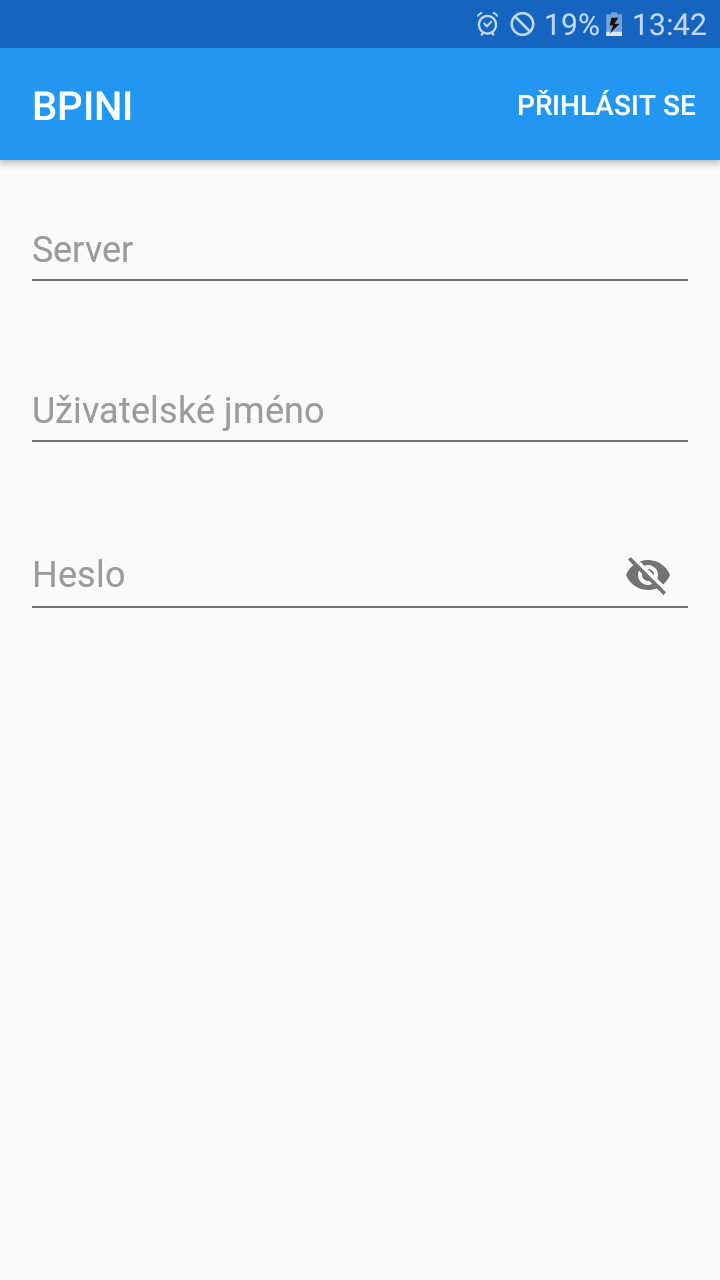
\includegraphics[width=\textwidth]{../images/client_android/Screenshot_20170610-134211.png}	
	\caption{Prázdný}
	\label{fig:Screenshot_20170610-134211}
  \end{subfigure}
  %
  \begin{subfigure}[b]{0.3\textwidth}
    \centering
	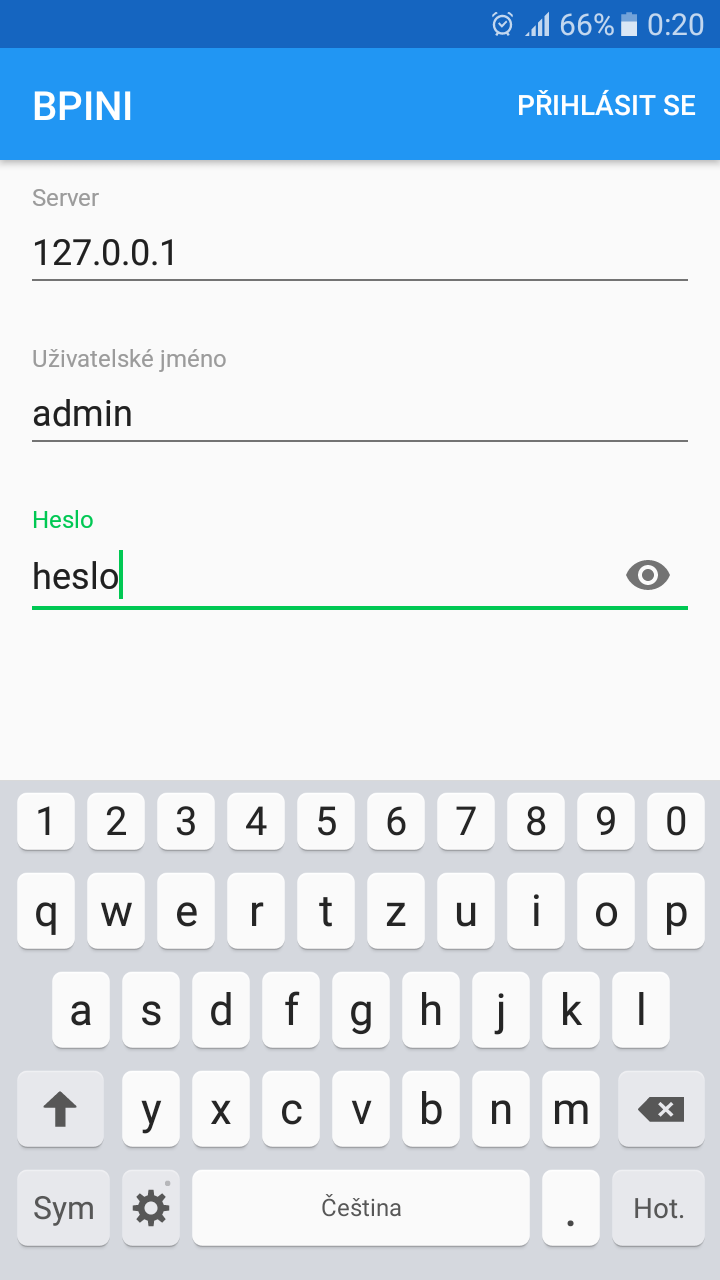
\includegraphics[width=\textwidth]{../images/client_android/Screenshot_20170612-002041.png}	
	\caption{Vyplněný}
	\label{fig:Screenshot_20170612-002041}
  \end{subfigure}
  \caption{Přihlašovací formulář}
\end{figure}


\section{Menu}
Menu se zobrazí stisknutím hamburger menu nebo vysunutím zpoza okraje (viz obrázky \ref{fig:Screenshot_20180412-020603}, \ref{fig:Screenshot_20180412-1523491587} a \ref{fig:Screenshot_20180412-023541}).
První položka menu otevírá detail přihlášeného uživatele, pak následují \uv{Položky}. 
Další položkou v menu jsou buď \uv{Tagy} nebo \uv{Čtečka}, zobrazení záleží na dostupnosti \texttt{NFC}, zařízením s \texttt{NFC} se zobrazí \uv{Čtečka} ostatním se jinak zobrazí \uv{Tagy}.
Poté následují \uv{Zařízení} a \uv{Uživatelé}, které jsou přístupné jen pro administrátora.
Poslední je \uv{O aplikaci}, zobrazí verzi, popis a autora aplikace.



\begin{figure}[H]
	\centering
  \begin{subfigure}[b]{0.3\textwidth}
    \centering
	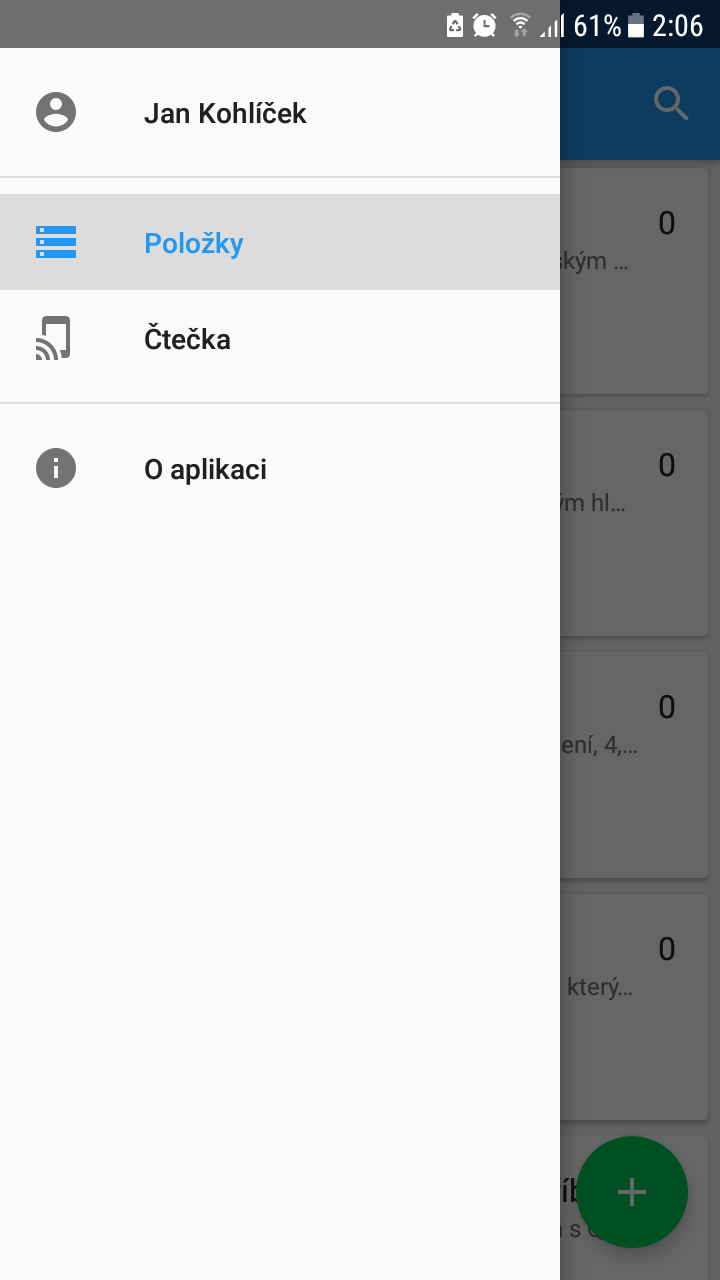
\includegraphics[width=\textwidth]{../images/client_android/Screenshot_20180412-020603.png}	
	\caption{Pro zařízení s \texttt{NFC}}
	\label{fig:Screenshot_20180412-020603}
  \end{subfigure}
  %
  \begin{subfigure}[b]{0.32\textwidth}
    \centering
	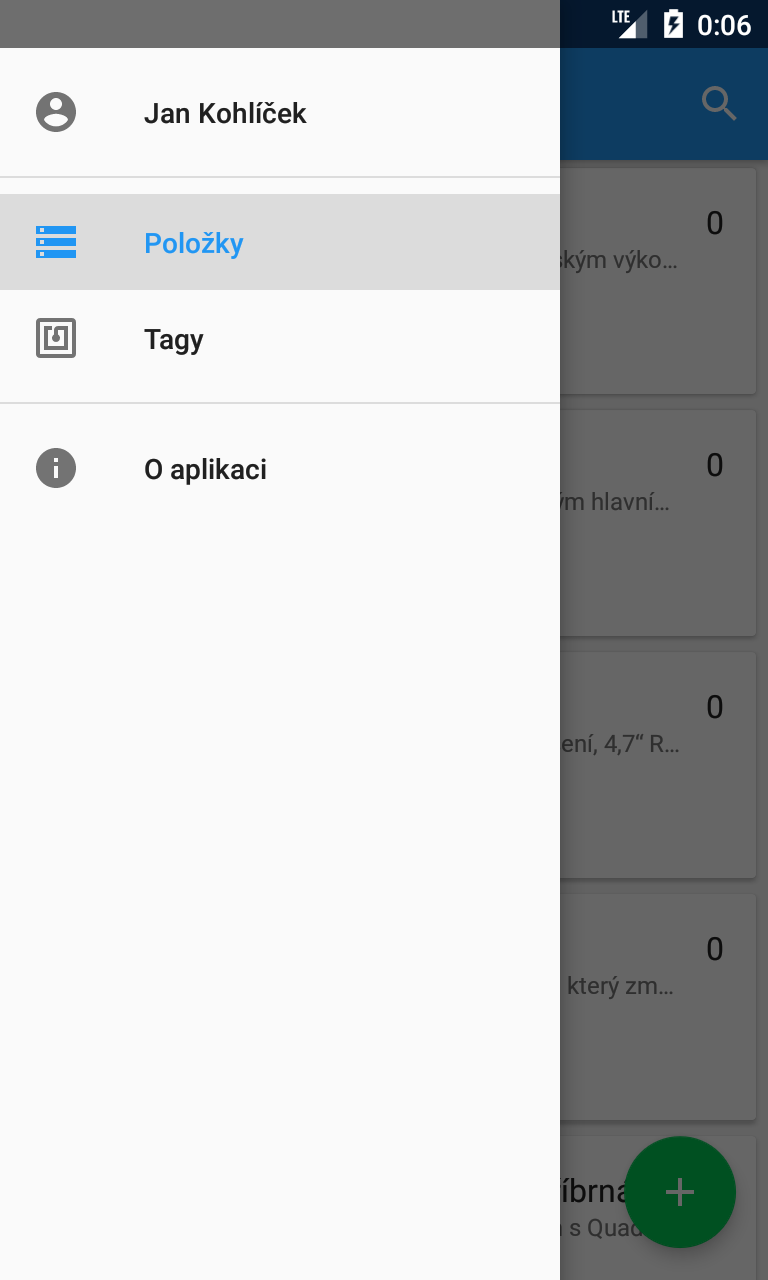
\includegraphics[width=\textwidth]{../images/client_android/Screenshot_20180412-1523491587.png}	
	\caption{Pro zařízení bez \texttt{NFC}}
	\label{fig:Screenshot_20180412-1523491587}
  \end{subfigure}
  %
  \begin{subfigure}[b]{0.3\textwidth}
    \centering
	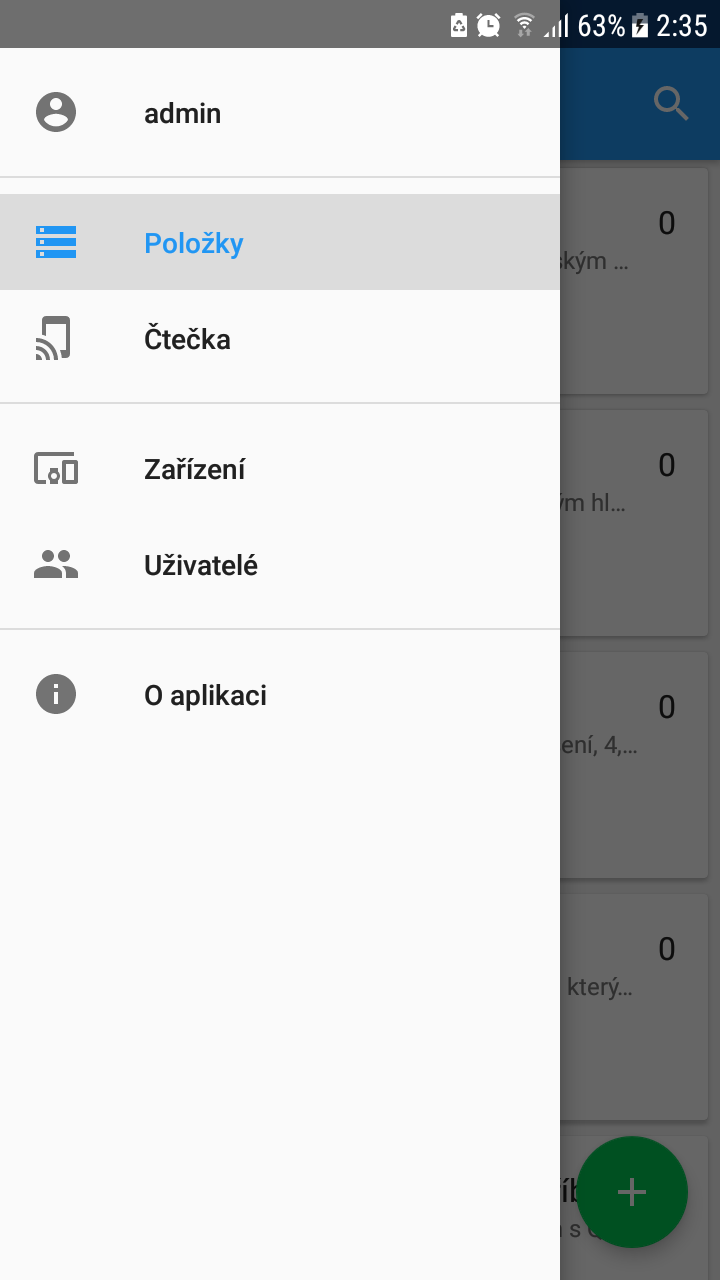
\includegraphics[width=\textwidth]{../images/client_android/Screenshot_20180412-023541.png}	
	\caption{Pro administrátora}
	\label{fig:Screenshot_20180412-023541}
  \end{subfigure}
  \caption{Menu aplikace}
\end{figure}



\section{Položky}	
Po spuštění aplikace se zobrazí seznam položek skladu (viz obrázek \ref{fig:Screenshot_20180412-030432}).
Položky můžete přidat pomocí zeleného plus v pravém dolním rohu a kliknutím na danou položku editovat.
Položku lze smazat jen tehdy, když se její počet rovná nule.
\begin{figure}[H]
	\centering
  \begin{subfigure}[b]{0.3\textwidth}
    \centering
	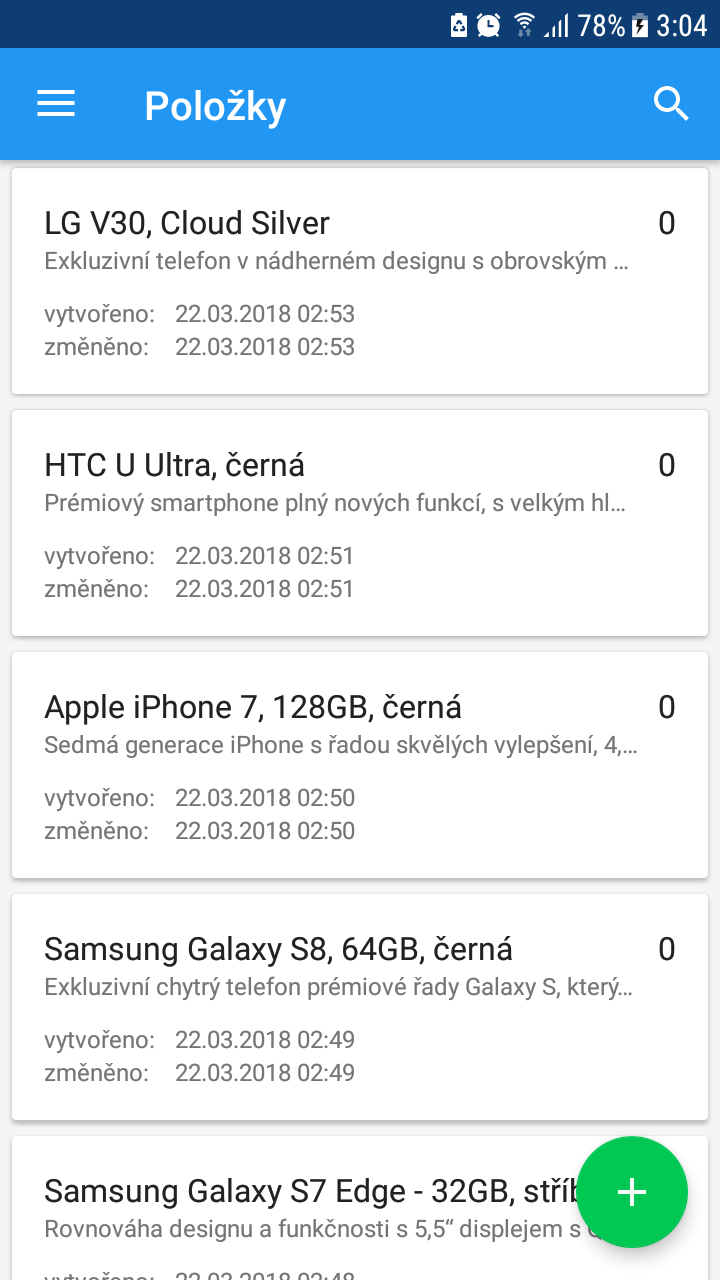
\includegraphics[width=\textwidth]{../images/client_android/Screenshot_20180412-030432.png}	
	\caption{Seznam položek}
	\label{fig:Screenshot_20180412-030432}
  \end{subfigure}
  %
  \begin{subfigure}[b]{0.3\textwidth}
    \centering
	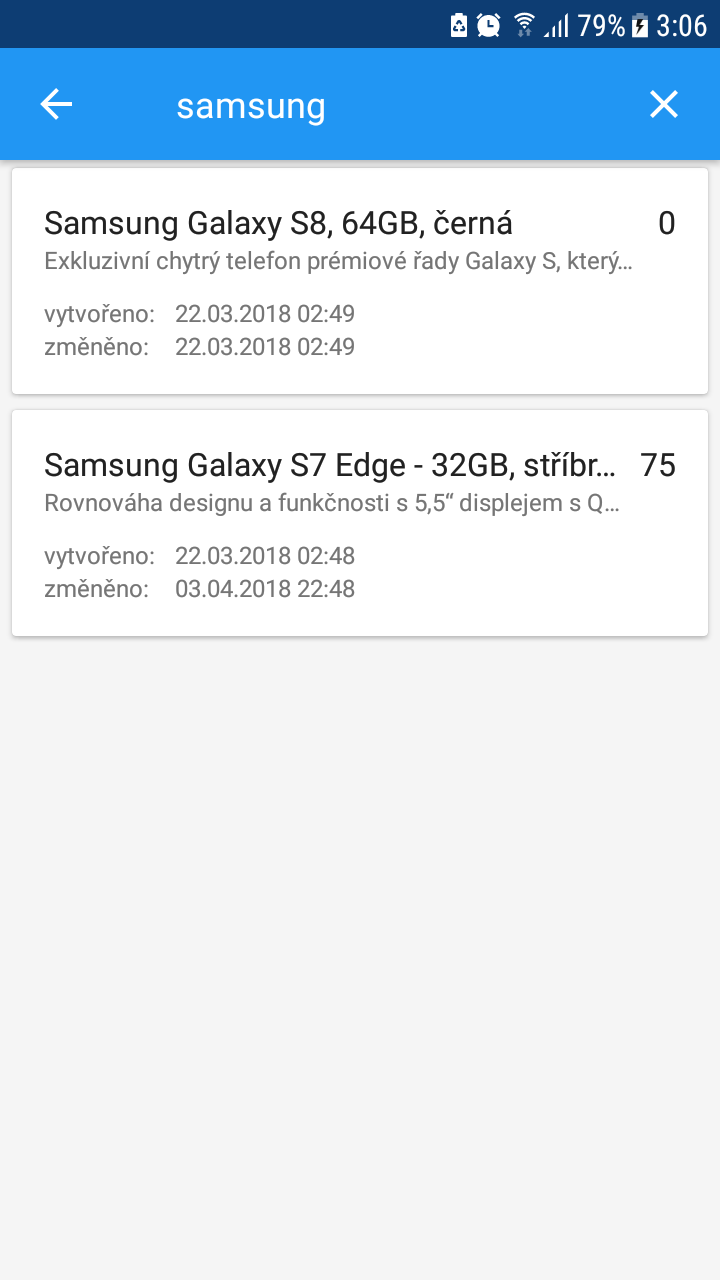
\includegraphics[width=\textwidth]{../images/client_android/Screenshot_20180412-030648.png}	
	\caption{Vyhledání položky}
	\label{fig:Screenshot_20180412-030648}
  \end{subfigure}
  %
  \begin{subfigure}[b]{0.3\textwidth}
    \centering
	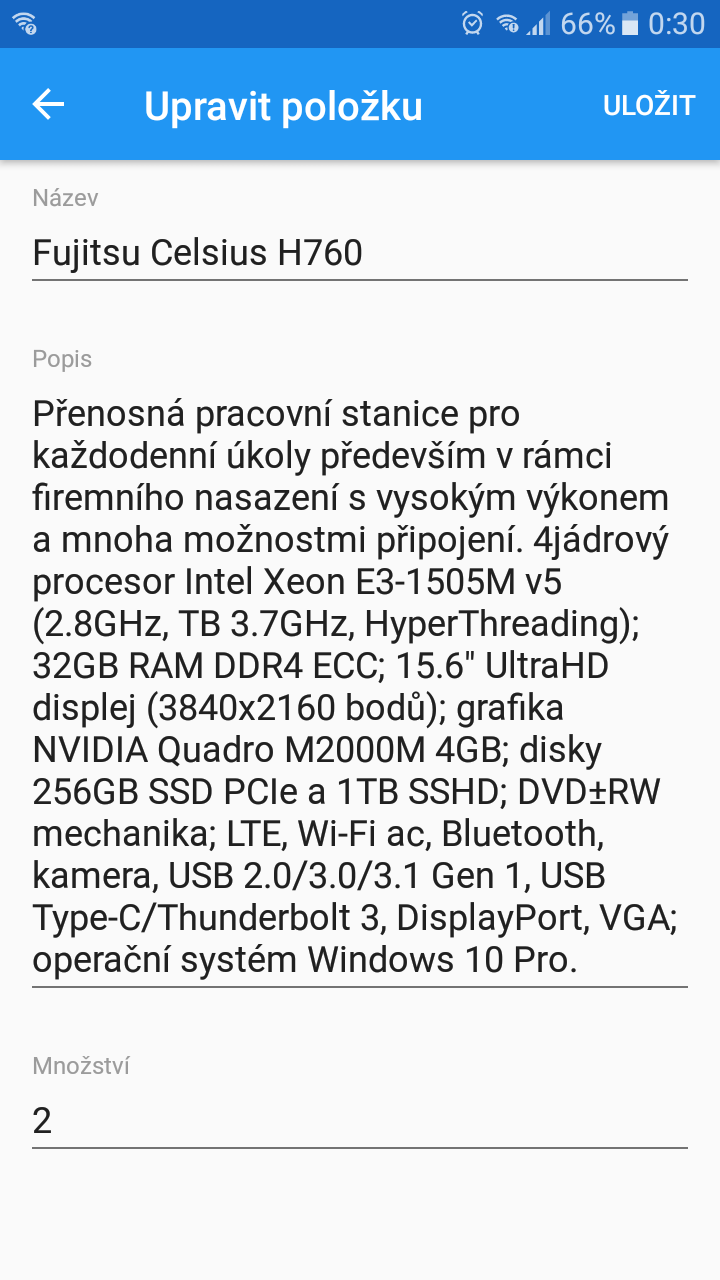
\includegraphics[width=\textwidth]{../images/client_android/Screenshot_20170612-003030.png}	
	\caption{Úprava položky}
	\label{fig:Screenshot_20170612-003030}
  \end{subfigure}
  \caption{Položky}
\end{figure}



\section{Tagy}
Tagy nelze přidávat ručně, jen pomocí čtečky. Kliknutím na tag se zobrazí editace (viz obrázek \ref{fig:Screenshot_20180412-031459}), která nabízí změnu typu. Tag může být tří typů:
\begin{description}
\item [neznámý] - tag nemá nastavenou žádnou funkci
\item [režim] - tag umožňuje čtečce RFID přepínat režimy přidat/odebrat položku
\item [položka] - tag reprezentuje položku ve skladu 
\end{description}
\begin{figure}[H]
	\centering
  \begin{subfigure}[b]{0.3\textwidth}
    \centering
	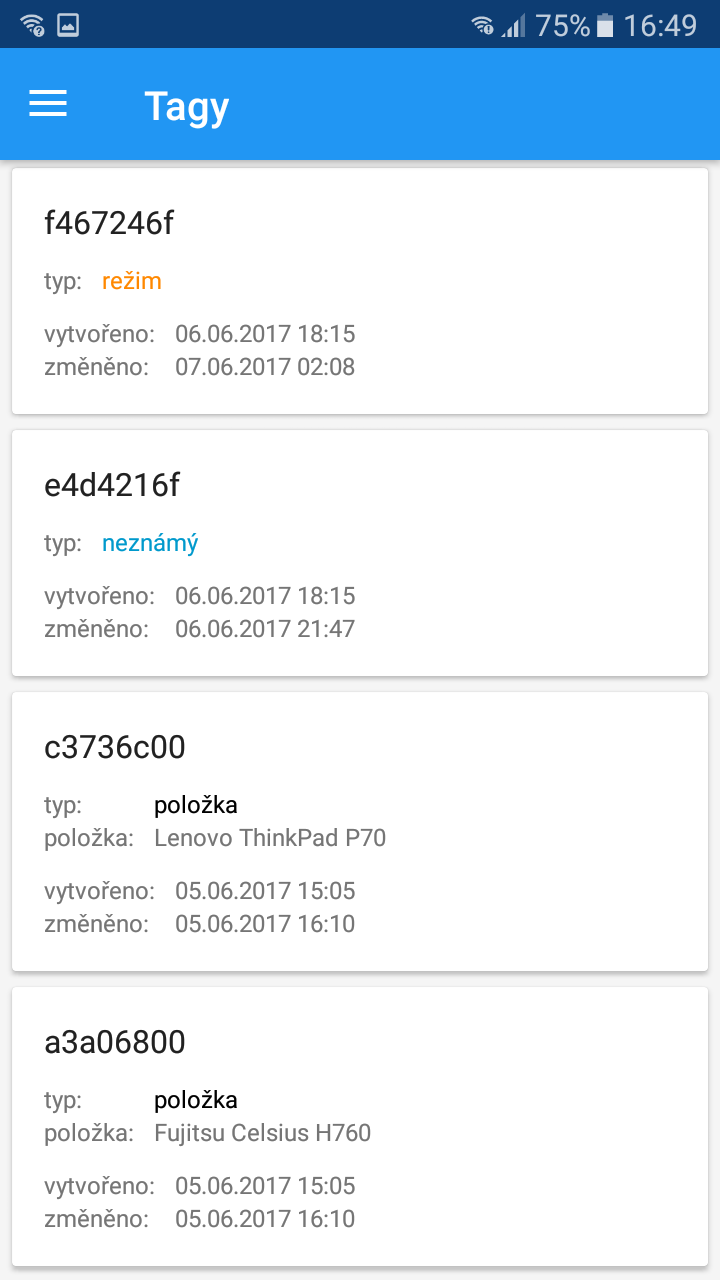
\includegraphics[width=\textwidth]{../images/client_android/Screenshot_20170607-164958.png}	
	\caption{Seznam tagů}
	\label{fig:Screenshot_20170607-164958}
  \end{subfigure}
  %
  \begin{subfigure}[b]{0.3\textwidth}
    \centering
	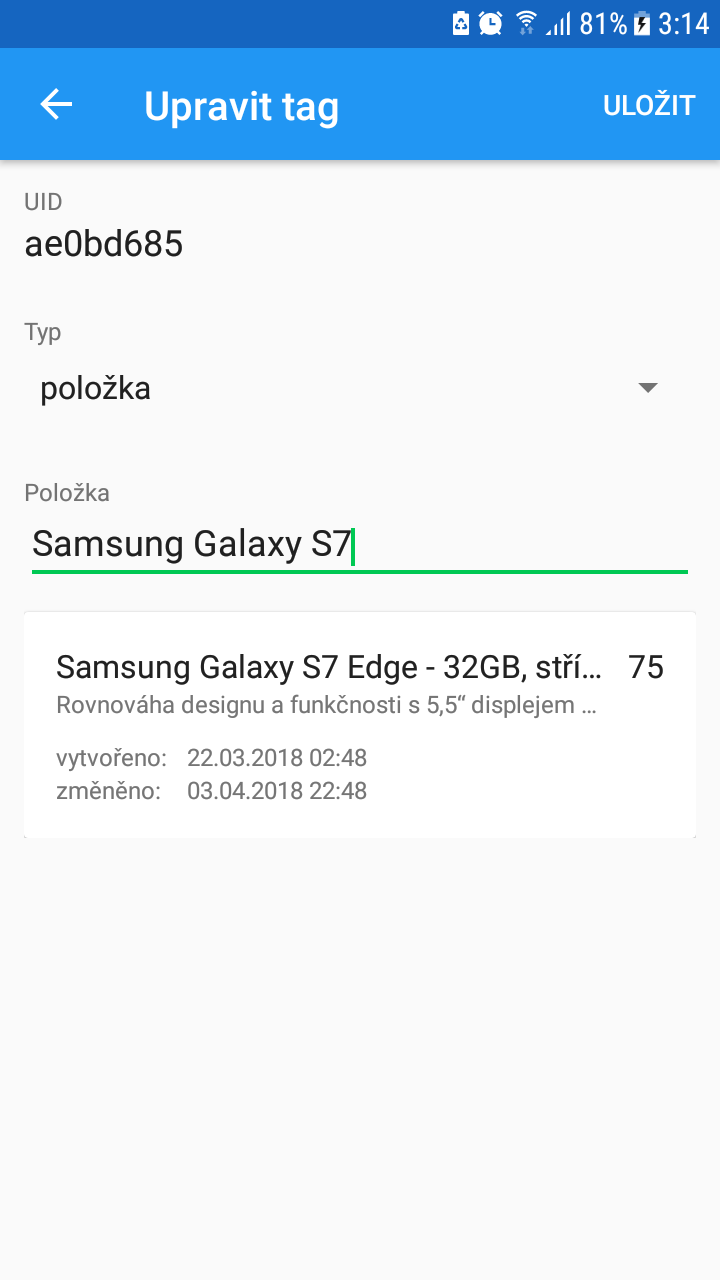
\includegraphics[width=\textwidth]{../images/client_android/Screenshot_20180412-031459.png}	
	\caption{Úprava tagu}
	\label{fig:Screenshot_20180412-031459}
  \end{subfigure}
  \caption{Tagy}
\end{figure}


\section{Čtečka}
Čtečka čekající na přiložení tagu (viz obrázek \ref{fig:Screenshot_20170607-165058}).
Po přiložení tagu se načtou detailní informace (viz obrázek \ref{fig:Screenshot_20170607-165117}), ale pokud není v systému zaevidován, pak je vytvořen tag typu \uv{neznámý}.
\begin{figure}[H]
	\centering
  \begin{subfigure}[b]{0.3\textwidth}
    \centering
	
\includegraphics[width=\textwidth]{../images/client_android/Screenshot_20170607-165058.png}	
	\caption{Připravená čtečka}
	\label{fig:Screenshot_20170607-165058}
  \end{subfigure}
  %
  \begin{subfigure}[b]{0.3\textwidth}
    \centering
	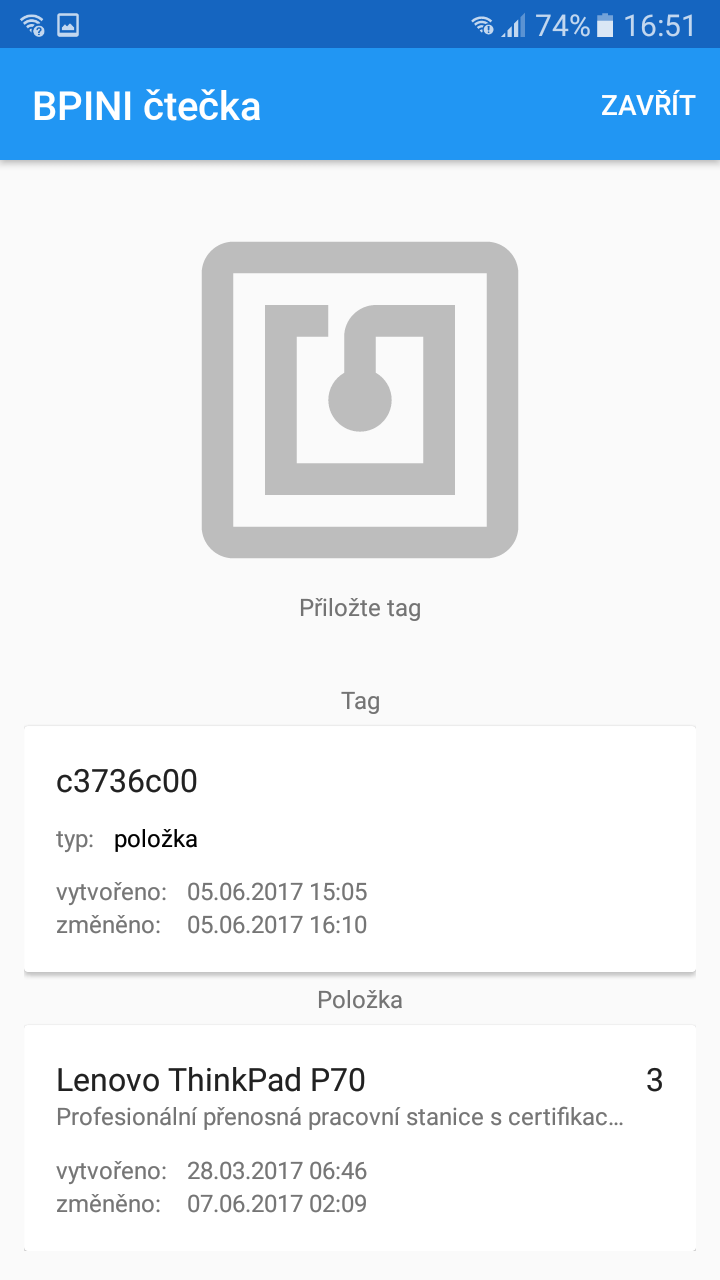
\includegraphics[width=\textwidth]{../images/client_android/Screenshot_20170607-165117.png}	
	\caption{Načtený tag}
	\label{fig:Screenshot_20170607-165117}
  \end{subfigure}
  \caption{Čtečka}
\end{figure}


\section{Administrace}
Seznam zařízení se ukazuje jen administrátorům (viz obrázek \ref{fig:Screenshot_20170607-165221}). Zařízení se evidují automaticky při jakémkoli pokusu o připojení k serveru. Aby se zařízení připojilo, je nutné, aby konkrétnímu zařízení byl povolen přístup. Ten se mění pomocí přepínače.
\begin{figure}[H]
	\centering
	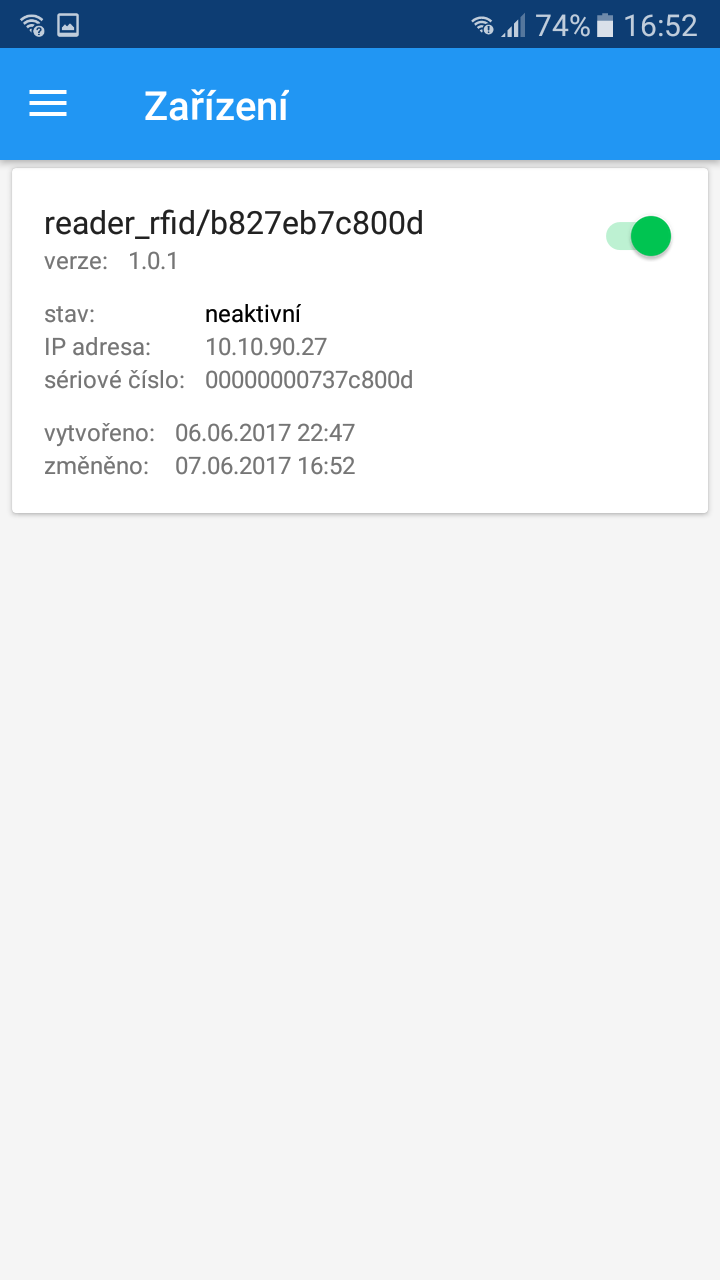
\includegraphics[width=0.3\textwidth]{../images/client_android/Screenshot_20170607-165221.png}	
	\caption{Zařízení}
	\label{fig:Screenshot_20170607-165221}
\end{figure}
\ \\
Jen administrátor má přístup ke správě uživatelů (viz obrázek \ref{fig:Screenshot_20170607-165248}).
Dostat se na vytvoření nového uživatele je možné přes zelené plus v pravém dolním rohu a kliknutím na uživatele editovat.
Uživatele s rolí \uv{administrátor} může vytvářet a editovat jen výchozí administrátor.
\begin{figure}[H]
	\centering
  \begin{subfigure}[b]{0.3\textwidth}
	\centering
	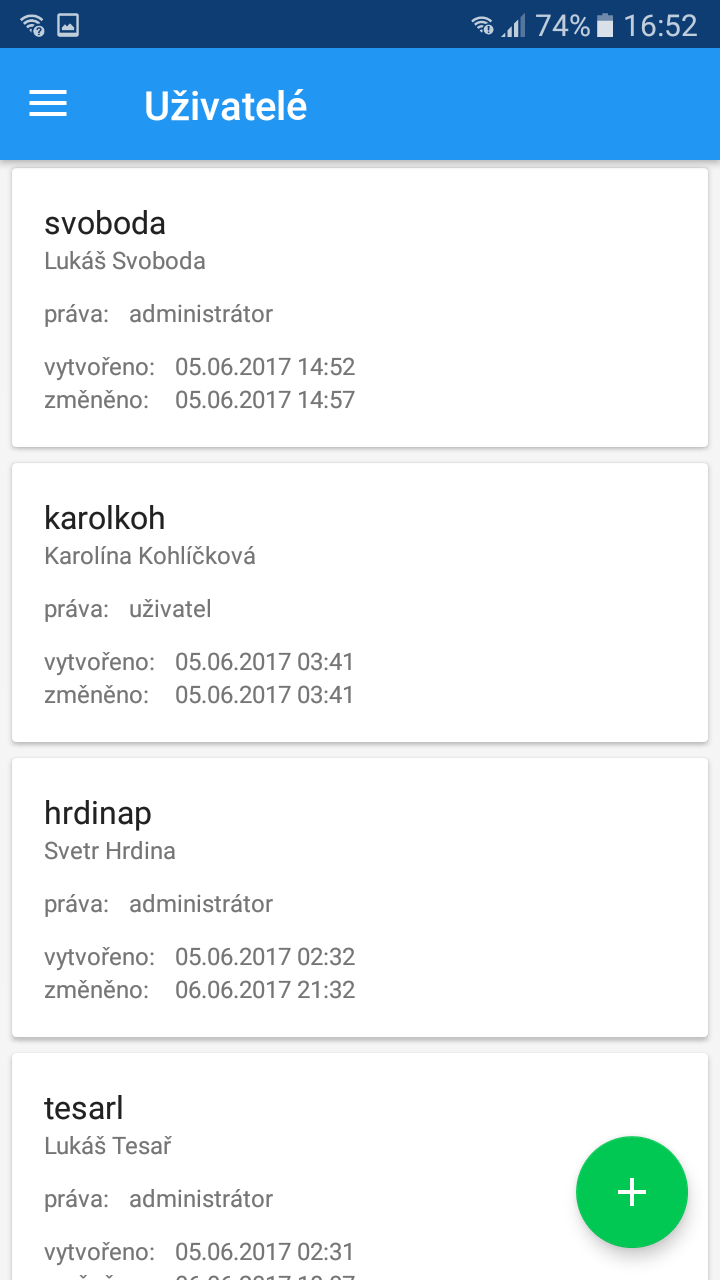
\includegraphics[width=\textwidth]{../images/client_android/Screenshot_20170607-165248.png}	
	\caption{Seznam uživatelů}
	\label{fig:Screenshot_20170607-165248}
  \end{subfigure}
  %
  \begin{subfigure}[b]{0.3\textwidth}
    \centering
	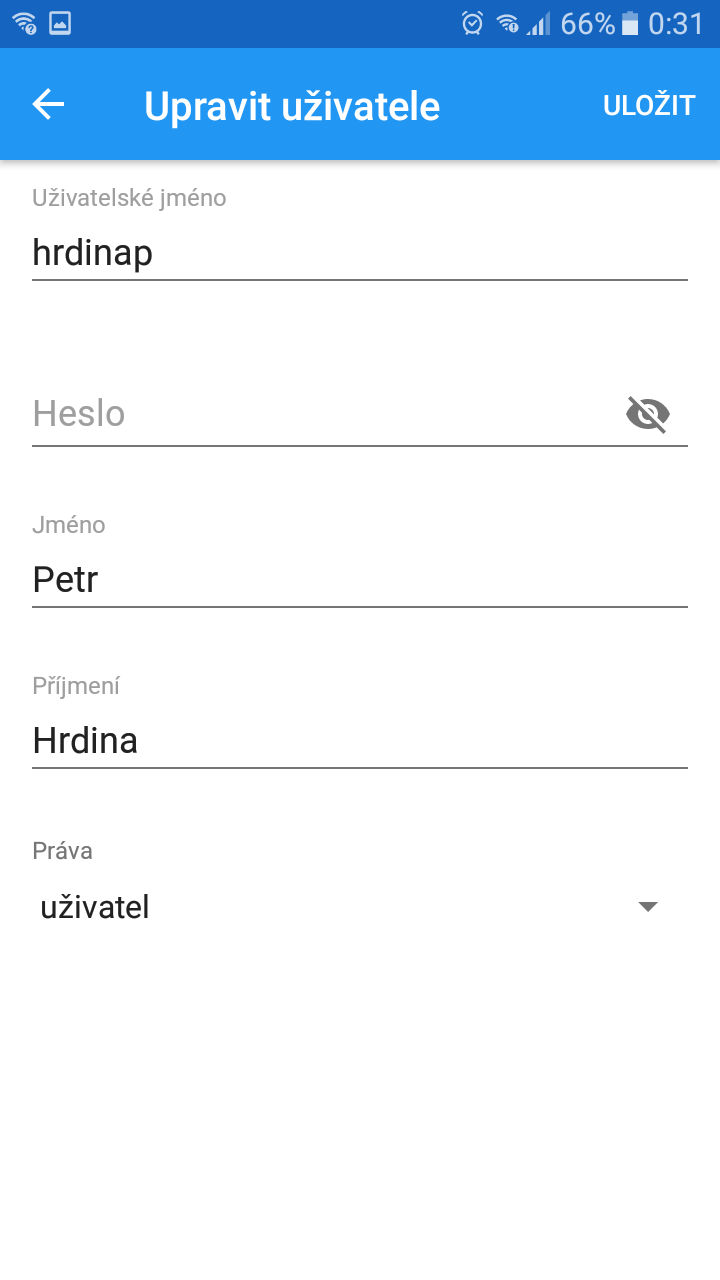
\includegraphics[width=\textwidth]{../images/client_android/Screenshot_20170612-003127.png}	
	\caption{Úprava uživatele}
	\label{fig:Screenshot_20170612-003127}
  \end{subfigure}
  \caption{Uživatelé}
\end{figure}


\chapter{Postup nasazení}
Projekt naleznete ke stažení na: \\ \url{https://github.com/kohlicekjan/BPINI} 

\section{Server}

\subsection{Instalace}
Pro spuštění serveru je potřeba nainstalovat \texttt{Node.js}. Na oficiálních stránkách je k dispozici podrobný postup: \\
\url{https://nodejs.org/en/download/package-manager/}
\\\\
Pro nainstalování potřebných modulů, spusťte ve složce \texttt{/src/Server/} tento příkaz:
\begin{verbatim}
npm install
\end{verbatim}
\ \\
Nainstalujte také databázi \texttt{MongoDB}, postup naleznete zde: \\
\url{https://docs.mongodb.com/manual/installation/}

\subsection{Konfigurace}
Ve složce projektu \texttt{/src/Server/config} jsou konfigurační soubory. 
V souboru \texttt{default.js} zadejte do \texttt{uri} adresu spuštěné databáze s názvem databáze, kterou chcete vytvořit.
Dále také můžete nastavit adresu a porty serveru. Ukázka konfigurace:
\begin{verbatim}
{
    host: '127.0.0.1',
    port: {
        http: 80,
        https: 443,
        mqtt: 1883
    },
    mongodb: {
        uri: 'mongodb://127.0.0.1:27017/warehouse'
    }
}
\end{verbatim}



\subsection{Spuštění}
Server spustíte tímto příkazem:
\begin{verbatim}
node server.js
\end{verbatim}


\section{Mobilní aplikace}
Aplikace je určena pro \texttt{Android 6.0} a vyšší.	
Soubor \texttt{BPINI-1.6.2.apk} nahrajte do mobilního zařízení a spusťte instalaci.
Při instalaci bude potřeba dočasně povolit \texttt{instalaci z neznámých zdrojů}.
Po dokončení najdete aplikaci v menu mezi ostatními aplikacemi.


\chapter{Testování}
Aplikace byla testovaná na zařízení \texttt{Samsung A3 (2017)} s \texttt{Androidem 7.0.0}, vše fungovalo správně.

\chapter{Závěr}
V rámci semestralní práce jsem také musel upravit \texttt{REST API}, což zkomplikovalo a zdrželo vývoj jednoduchých rozšíření.

Změna protokolu pro autentizaci na \texttt{OAuth 2.0} se mi nepovedlo, alespoň jsem přešel na šifrovanou komunikaci, která je dnes standardem.

Vyhledání je plně funkční, jen škoda chybějícího fulltextu, to ale budu řešit na straně \texttt{REST API}.

Změna propojení mezi položkou skladu a tagem se více měně povedlo. Použil jsem \texttt{AutoCompleteTextView} na našepatávač názvu skladové položky, pokud existuje jen jedna schoda zobrazí se detail skladové položky a umožní se uložení. Možný problém může stat u skladových položek se stejným názvem, tento problém zatím nevím, jak budu řešit.

Dále jsem opravil chybu s automatickým vracením zpět při neočekávané chybě od severu.
Další chybou bylo možnost spustit \uv{Čtečka}, aniž by byl uživatel přihlášený.

Také jsem přidal automatické odhlášení uživatele, při spuštění aplikace s vyšší vezí než když se přihlašoval. Touhle funčností se předchazí chybám z nekonzistence dat mezi verzema. 

Do budoucna plánuji možnost zobrazit archiv všech změn daného záznamu. Pak přidám cenu zboží ke kterému je zapotřebí i měna. Pro uživatelé s jinou měnou se bude cena přepočítávat podle aktuálního kurzu. Přidat cenu zboží nebude jednoduchá záležitost.

\end{document}